\chapter{Durchführung des Versuchs}

\section*{Aufgabe 1: Bestimmung der Faraday-Konstante durch Kupferabscheidung}
Für die erste Aufgabe wird die Elektrolyse einer Kupfersulfatlösung (CuSO$_4$) durchgeführt. Die Kupferplatten werden vor Versuchsbeginn gründlich gereinigt (Schmirgeln, Spülen mit Wasser) und getrocknet. Anschließend erfolgt eine genaue Wägung, um die Ausgangsmasse zu bestimmen. Die Kupferplatten werden in die Lösung getaucht, und der Strom über den Schiebewiderstand auf etwa 0,5–1\,A eingestellt. Die Stromstärke ist regelmäßig zu kontrollieren und ggf. anzupassen.  

Während der Elektrolyse fließt der Strom mindestens 30\,Minuten. Vor Beginn ist zu überlegen, welche Stromstärke gewählt werden soll, und diese nach Einschalten des Netzteils schnellstmöglich zu regulieren. Bei plötzlichen Stromänderungen, die sich nicht korrigieren lassen, ist der Assistent zu informieren.  

Nach Abschluss der Elektrolyse werden die Kupferplatten vorsichtig mit Wasser gespült, um eine Ablösung von Kupfer zu vermeiden. Anschließend werden sie mit dem Fön getrocknet und erneut gewogen. Die Masseänderungen der Elektroden ermöglichen die Berechnung der Faraday-Konstante $F$ über das erste Faraday’sche Gesetz in \hyperref[eq:first_faraday]{Gleichung \ref*{eq:first_faraday}}. Die transportierte Ladung $Q$ kann aus \hyperref[eq:ladung]{Gleichung \ref*{eq:ladung}} bestimmt werden, und die Dissoziation von CuSO$_4$ wird durch \hyperref[eq:cu_dissoziation]{Gleichung \ref*{eq:cu_dissoziation}} beschrieben.
\begin{figure}[h!]
    \vspace{1.75cm}
    \includegraphics[width=0.48\textwidth, page=1]{img/21/21-Versuchsaufbau-num.pdf}
    \caption{Versuchsaufbau zur Elektrolyse mit Kupfer. 1: Strom- bzw. Spannungsquelle. 2: Schiebwiderstand. 3: Elektrolyse-Gemisch. 4: Stoppuhr. 5: Kathoden-Stomversorgung. 6: Anoden-Stomversorgung. 7: Kupfer-Kathode. 8: Kupfer-Anode}
    \label{fig:log_gezeichnet}
\end{figure}


\section*{Aufgabe 2: Bestimmung der Faraday-Konstante durch Wasserzersetzung}

Für die zweite Aufgabe wird ein Hoffmannscher Wasserzersetzungsapparat verwendet. Die beiden Schenkel werden vollständig mit Flüssigkeit gefüllt, indem das Vorratsgefäß langsam angehoben wird, bis der Flüssigkeitsspiegel leicht über den Hähnen liegt. Anschließend werden die Hähne wieder geschlossen.  

Der Apparat wird ohne Schiebewiderstand direkt an das Netzteil angeschlossen. Während eines kurzen Vorlaufs (ca. 30\,s) wird der Strom auf einen festen Wert von $I = 0,5$–$0,9$\,A eingestellt. Dazu den Stromregler auf 0\,A und den Spannungsregler auf den rechten Anschlag stellen, dann den Strom auf den gewünschten Wert erhöhen. Nach Wartezeit, bis alle Gasbläschen aufgestiegen sind, werden die Startvolumina in beiden Röhren notiert.  

Der Strom soll solange fließen, bis der Wasserstoff eine Röhre zu etwa 3/4 füllt. Die benötigte Zeit wird gemessen. Die Stromstärke ist etwa jede Minute auf Konstanz zu kontrollieren, entweder durch Nachregeln oder durch spätere Mittelung. Die Gasvolumina in beiden Röhren werden abgelesen, indem das Vorratsgefäß vorsichtig gesenkt wird, bis die Flüssigkeitsspiegel in den Schenkeln und im Vorratsgefäß gleich hoch stehen. Dieser Messaufbau stellt sicher, dass der Hydrostatik-Druck korrekt berücksichtigt wird (vgl. \hyperref[eq:druck]{Gleichung \ref*{eq:druck}}).  

Die gemessenen Gasvolumina von Wasserstoff und Sauerstoff erlauben die Berechnung der Faraday-Konstante $F$ über \hyperref[eq:stoffmenge]{Gleichung \ref*{eq:stoffmenge}}, wobei das Molvolumen $V_\mathrm{Mol}$ gemäß \hyperref[eq:molvolumen]{Gleichung \ref*{eq:molvolumen}} berechnet wird. Die elektrochemischen Reaktionen an der Kathode und Anode sind in \hyperref[eq:h2_kathode]{Gleichung \ref*{eq:h2_kathode}} und \hyperref[eq:o2_anode]{Gleichung \ref*{eq:o2_anode}} dargestellt.

\begin{figure}[h!]
    \vspace{1.75cm}
    \includegraphics[width=0.48\textwidth, page=2]{img/21/21-Versuchsaufbau-num.pdf}
    \caption{Versuchsaufbau zur Wasserelektrolyse. 1: Wasserschwefelsäurengemisch. 2: Kathoden-Schenkel (Wasserstoff). 3: Anoden-Schenkel (Sauerstoff). 4: Kathoden-Stromverbindung. 5: Anoden-Stromverbindung. 6: Strom- bzw. Spannungsquelle.}
    \label{fig:log_gezeichnet}
\end{figure}

\section*{Aufgabe 3: Qualitative Beobachtung der Umkehrung der Elektrolyse in einer Brennstoffzelle}

In der dritten Aufgabe wird das Prinzip einer PEM-Brennstoffzelle qualitativ untersucht. Dabei erfolgt die Reaktion von Wasserstoff mit Sauerstoff zu Wasser kontrolliert und „kalt“ ohne offene Verbrennung. An der Anode wird Wasserstoff in Protonen und Elektronen gespalten (\hyperref[eq:h2_anode]{Gleichung \ref*{eq:h2_anode}}), die Protonen passieren die Membran zur Kathode, und die Elektronen fließen über einen äußeren Stromkreis. An der Kathode reagieren Protonen, Elektronen und Sauerstoff zu Wasser (\hyperref[eq:h2o_kathode]{Gleichung \ref*{eq:h2o_kathode}}). Durch diesen Prozess kann elektrische Energie gewonnen werden, während die elektrochemische Reaktion kontrolliert abläuft.
\begin{figure}[t]
    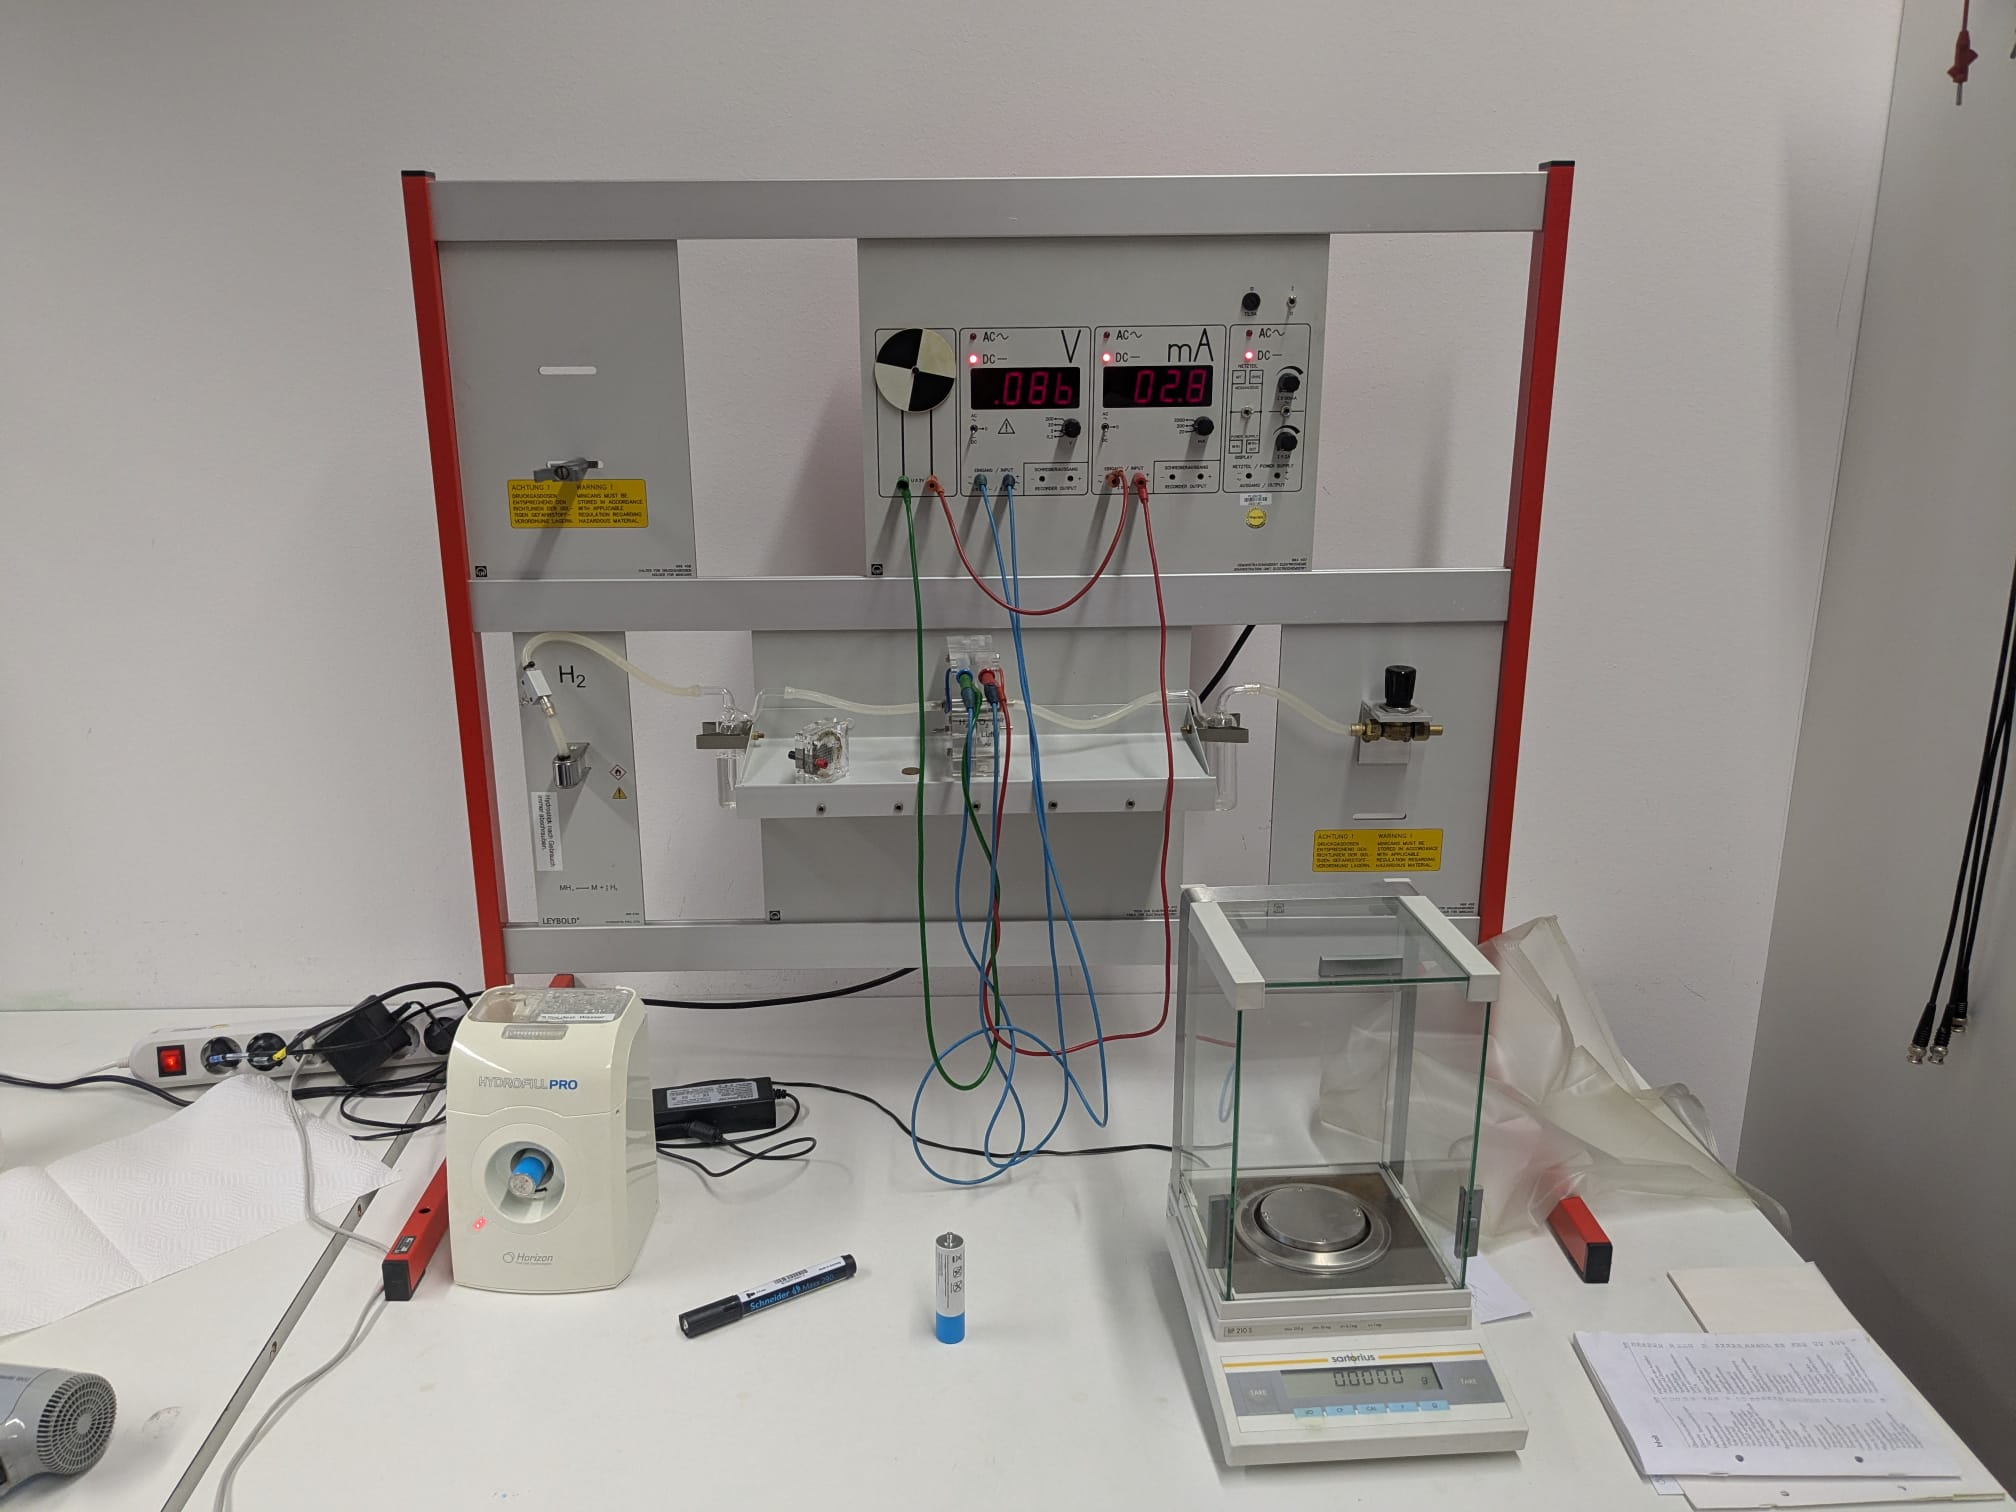
\includegraphics[width=0.5\textwidth]{img/21/Elektrolyse_Bild.jpg}
    \caption{Versuchsaufbau der Wasserstoffbrennzelle. Auch zusehen die Präzisions-Waage.}
    \label{fig:log_gezeichnet}
\end{figure}